% Options for packages loaded elsewhere
\PassOptionsToPackage{unicode}{hyperref}
\PassOptionsToPackage{hyphens}{url}
%
\documentclass[
]{book}
\usepackage{lmodern}
\usepackage{amsmath}
\usepackage{ifxetex,ifluatex}
\ifnum 0\ifxetex 1\fi\ifluatex 1\fi=0 % if pdftex
  \usepackage[T1]{fontenc}
  \usepackage[utf8]{inputenc}
  \usepackage{textcomp} % provide euro and other symbols
  \usepackage{amssymb}
\else % if luatex or xetex
  \usepackage{unicode-math}
  \defaultfontfeatures{Scale=MatchLowercase}
  \defaultfontfeatures[\rmfamily]{Ligatures=TeX,Scale=1}
\fi
% Use upquote if available, for straight quotes in verbatim environments
\IfFileExists{upquote.sty}{\usepackage{upquote}}{}
\IfFileExists{microtype.sty}{% use microtype if available
  \usepackage[]{microtype}
  \UseMicrotypeSet[protrusion]{basicmath} % disable protrusion for tt fonts
}{}
\makeatletter
\@ifundefined{KOMAClassName}{% if non-KOMA class
  \IfFileExists{parskip.sty}{%
    \usepackage{parskip}
  }{% else
    \setlength{\parindent}{0pt}
    \setlength{\parskip}{6pt plus 2pt minus 1pt}}
}{% if KOMA class
  \KOMAoptions{parskip=half}}
\makeatother
\usepackage{xcolor}
\IfFileExists{xurl.sty}{\usepackage{xurl}}{} % add URL line breaks if available
\IfFileExists{bookmark.sty}{\usepackage{bookmark}}{\usepackage{hyperref}}
\hypersetup{
  pdftitle={Bygge statistiske modeller med kategoriske prediktorvariabler (t-tester, ANOVA)},
  pdfauthor={Christian Magelssen},
  hidelinks,
  pdfcreator={LaTeX via pandoc}}
\urlstyle{same} % disable monospaced font for URLs
\usepackage{color}
\usepackage{fancyvrb}
\newcommand{\VerbBar}{|}
\newcommand{\VERB}{\Verb[commandchars=\\\{\}]}
\DefineVerbatimEnvironment{Highlighting}{Verbatim}{commandchars=\\\{\}}
% Add ',fontsize=\small' for more characters per line
\usepackage{framed}
\definecolor{shadecolor}{RGB}{248,248,248}
\newenvironment{Shaded}{\begin{snugshade}}{\end{snugshade}}
\newcommand{\AlertTok}[1]{\textcolor[rgb]{0.94,0.16,0.16}{#1}}
\newcommand{\AnnotationTok}[1]{\textcolor[rgb]{0.56,0.35,0.01}{\textbf{\textit{#1}}}}
\newcommand{\AttributeTok}[1]{\textcolor[rgb]{0.77,0.63,0.00}{#1}}
\newcommand{\BaseNTok}[1]{\textcolor[rgb]{0.00,0.00,0.81}{#1}}
\newcommand{\BuiltInTok}[1]{#1}
\newcommand{\CharTok}[1]{\textcolor[rgb]{0.31,0.60,0.02}{#1}}
\newcommand{\CommentTok}[1]{\textcolor[rgb]{0.56,0.35,0.01}{\textit{#1}}}
\newcommand{\CommentVarTok}[1]{\textcolor[rgb]{0.56,0.35,0.01}{\textbf{\textit{#1}}}}
\newcommand{\ConstantTok}[1]{\textcolor[rgb]{0.00,0.00,0.00}{#1}}
\newcommand{\ControlFlowTok}[1]{\textcolor[rgb]{0.13,0.29,0.53}{\textbf{#1}}}
\newcommand{\DataTypeTok}[1]{\textcolor[rgb]{0.13,0.29,0.53}{#1}}
\newcommand{\DecValTok}[1]{\textcolor[rgb]{0.00,0.00,0.81}{#1}}
\newcommand{\DocumentationTok}[1]{\textcolor[rgb]{0.56,0.35,0.01}{\textbf{\textit{#1}}}}
\newcommand{\ErrorTok}[1]{\textcolor[rgb]{0.64,0.00,0.00}{\textbf{#1}}}
\newcommand{\ExtensionTok}[1]{#1}
\newcommand{\FloatTok}[1]{\textcolor[rgb]{0.00,0.00,0.81}{#1}}
\newcommand{\FunctionTok}[1]{\textcolor[rgb]{0.00,0.00,0.00}{#1}}
\newcommand{\ImportTok}[1]{#1}
\newcommand{\InformationTok}[1]{\textcolor[rgb]{0.56,0.35,0.01}{\textbf{\textit{#1}}}}
\newcommand{\KeywordTok}[1]{\textcolor[rgb]{0.13,0.29,0.53}{\textbf{#1}}}
\newcommand{\NormalTok}[1]{#1}
\newcommand{\OperatorTok}[1]{\textcolor[rgb]{0.81,0.36,0.00}{\textbf{#1}}}
\newcommand{\OtherTok}[1]{\textcolor[rgb]{0.56,0.35,0.01}{#1}}
\newcommand{\PreprocessorTok}[1]{\textcolor[rgb]{0.56,0.35,0.01}{\textit{#1}}}
\newcommand{\RegionMarkerTok}[1]{#1}
\newcommand{\SpecialCharTok}[1]{\textcolor[rgb]{0.00,0.00,0.00}{#1}}
\newcommand{\SpecialStringTok}[1]{\textcolor[rgb]{0.31,0.60,0.02}{#1}}
\newcommand{\StringTok}[1]{\textcolor[rgb]{0.31,0.60,0.02}{#1}}
\newcommand{\VariableTok}[1]{\textcolor[rgb]{0.00,0.00,0.00}{#1}}
\newcommand{\VerbatimStringTok}[1]{\textcolor[rgb]{0.31,0.60,0.02}{#1}}
\newcommand{\WarningTok}[1]{\textcolor[rgb]{0.56,0.35,0.01}{\textbf{\textit{#1}}}}
\usepackage{longtable,booktabs}
\usepackage{calc} % for calculating minipage widths
% Correct order of tables after \paragraph or \subparagraph
\usepackage{etoolbox}
\makeatletter
\patchcmd\longtable{\par}{\if@noskipsec\mbox{}\fi\par}{}{}
\makeatother
% Allow footnotes in longtable head/foot
\IfFileExists{footnotehyper.sty}{\usepackage{footnotehyper}}{\usepackage{footnote}}
\makesavenoteenv{longtable}
\usepackage{graphicx}
\makeatletter
\def\maxwidth{\ifdim\Gin@nat@width>\linewidth\linewidth\else\Gin@nat@width\fi}
\def\maxheight{\ifdim\Gin@nat@height>\textheight\textheight\else\Gin@nat@height\fi}
\makeatother
% Scale images if necessary, so that they will not overflow the page
% margins by default, and it is still possible to overwrite the defaults
% using explicit options in \includegraphics[width, height, ...]{}
\setkeys{Gin}{width=\maxwidth,height=\maxheight,keepaspectratio}
% Set default figure placement to htbp
\makeatletter
\def\fps@figure{htbp}
\makeatother
\setlength{\emergencystretch}{3em} % prevent overfull lines
\providecommand{\tightlist}{%
  \setlength{\itemsep}{0pt}\setlength{\parskip}{0pt}}
\setcounter{secnumdepth}{5}
\usepackage{booktabs}
\ifluatex
  \usepackage{selnolig}  % disable illegal ligatures
\fi
\usepackage[]{natbib}
\bibliographystyle{apalike}

\title{Bygge statistiske modeller med kategoriske prediktorvariabler (t-tester, ANOVA)}
\author{Christian Magelssen}
\date{2021-03-28}

\begin{document}
\maketitle

{
\setcounter{tocdepth}{1}
\tableofcontents
}
\hypertarget{intro}{%
\chapter{Introduksjon}\label{intro}}

I dette kapittelet skal vi lære å bygge statistiske modeller for å teste om \textbf{to eller flere grupper er forskjellige på en avhengig variabel som er kontinuerlig}.

En variabel sies å være \textbf{kontinuerlig} når vi kan bestemme hvor presist vi ønsker å måle det. For eksempel regnes tid som en kontuerlig variabel fordi det (i prinsippet) ikke er noen grenser hvor fint vi kan måle tid; vi kan måle det i år, måneder, uker, dager, timer, minutter, sekunder, tideler, hundredeler eller tusendeler.

\textbf{Grupper} defineres innenfor psykologifaget som en samling mennesker som deler bestemte karakterstikker. Det kan være spillere på et fotballag, individer på et treningssenter, eller menn og kvinner. Dette er også eksempler på grupper der inndelingen faller seg naturlig. I eksperimentelle studier er disse.

La oss se på hvordan en slik analyse vil se ut.

Reference a figure by its code chunk label with the \texttt{fig:} prefix, e.g., see Figure \ref{fig:nice-fig}. Similarly, you can reference tables generated from \texttt{knitr::kable()}, e.g., see Table \ref{tab:nice-tab}.

\begin{Shaded}
\begin{Highlighting}[]
\NormalTok{knitr}\SpecialCharTok{::}\FunctionTok{kable}\NormalTok{(}
  \FunctionTok{head}\NormalTok{(iris, }\DecValTok{20}\NormalTok{), }\AttributeTok{caption =} \StringTok{\textquotesingle{}Here is a nice table!\textquotesingle{}}\NormalTok{,}
  \AttributeTok{booktabs =} \ConstantTok{TRUE}
\NormalTok{)}
\end{Highlighting}
\end{Shaded}

\begin{table}

\caption{\label{tab:nice-tab}Here is a nice table!}
\centering
\begin{tabular}[t]{rrrrl}
\toprule
Sepal.Length & Sepal.Width & Petal.Length & Petal.Width & Species\\
\midrule
5.1 & 3.5 & 1.4 & 0.2 & setosa\\
4.9 & 3.0 & 1.4 & 0.2 & setosa\\
4.7 & 3.2 & 1.3 & 0.2 & setosa\\
4.6 & 3.1 & 1.5 & 0.2 & setosa\\
5.0 & 3.6 & 1.4 & 0.2 & setosa\\
\addlinespace
5.4 & 3.9 & 1.7 & 0.4 & setosa\\
4.6 & 3.4 & 1.4 & 0.3 & setosa\\
5.0 & 3.4 & 1.5 & 0.2 & setosa\\
4.4 & 2.9 & 1.4 & 0.2 & setosa\\
4.9 & 3.1 & 1.5 & 0.1 & setosa\\
\addlinespace
5.4 & 3.7 & 1.5 & 0.2 & setosa\\
4.8 & 3.4 & 1.6 & 0.2 & setosa\\
4.8 & 3.0 & 1.4 & 0.1 & setosa\\
4.3 & 3.0 & 1.1 & 0.1 & setosa\\
5.8 & 4.0 & 1.2 & 0.2 & setosa\\
\addlinespace
5.7 & 4.4 & 1.5 & 0.4 & setosa\\
5.4 & 3.9 & 1.3 & 0.4 & setosa\\
5.1 & 3.5 & 1.4 & 0.3 & setosa\\
5.7 & 3.8 & 1.7 & 0.3 & setosa\\
5.1 & 3.8 & 1.5 & 0.3 & setosa\\
\bottomrule
\end{tabular}
\end{table}

You can write citations, too. For example, we are using the \textbf{bookdown} package \citep{R-bookdown} in this sample book, which was built on top of R Markdown and \textbf{knitr} \citep{xie2015}.

\hypertarget{datasett-3-sett-vs.-1-sett}{%
\chapter{Datasett (3 sett vs.~1 sett)}\label{datasett-3-sett-vs.-1-sett}}

Et spørsmål mange treningsentusiaster lurer på er hvor mange serier som er best å gjennnomføre for å få maksimal treningseffekt i styrketrening. Noen mener at ett sett er tilstrekkelig, mens andre mener at et hardere treningstimuli er nødvendig og at to eller flere sett derfor er bedre. En forsker som var tidlig ute med å undersøke dette er deres egen Bent Rønnestad.

Eksperimentet ble gjennomført som et \textbf{between-subject design} med to grupper: en gruppe trente 1 sett på underkroppen og 3 sett på overkroppen; En annen gruppe trente 3 sett på underkroppen og 1 sett på overkroppen. Disse gruppene kalte han henholdsvis \textbf{1L-3U} og \textbf{3L-1U} (L=lower; U=Upper). De to gruppene trente 3 ganger i uken i totalt 11 uker. Forskerne ville så se hva som ga best fremgang på 1RM. Den avhengige variabelen ble derfor \%-fremgang på 1RM på underkroppsøvelser. De fant at 3L-1U hadde større fremgang enn 1L-3U fra pre til post (41 vs 21 \% endring). Denne forskjellen var signifikant ved en uavhengig t-test. Med andre ord kan det se ut til at det kan lønne seg å trene flere sett per styrketreningsøkt.

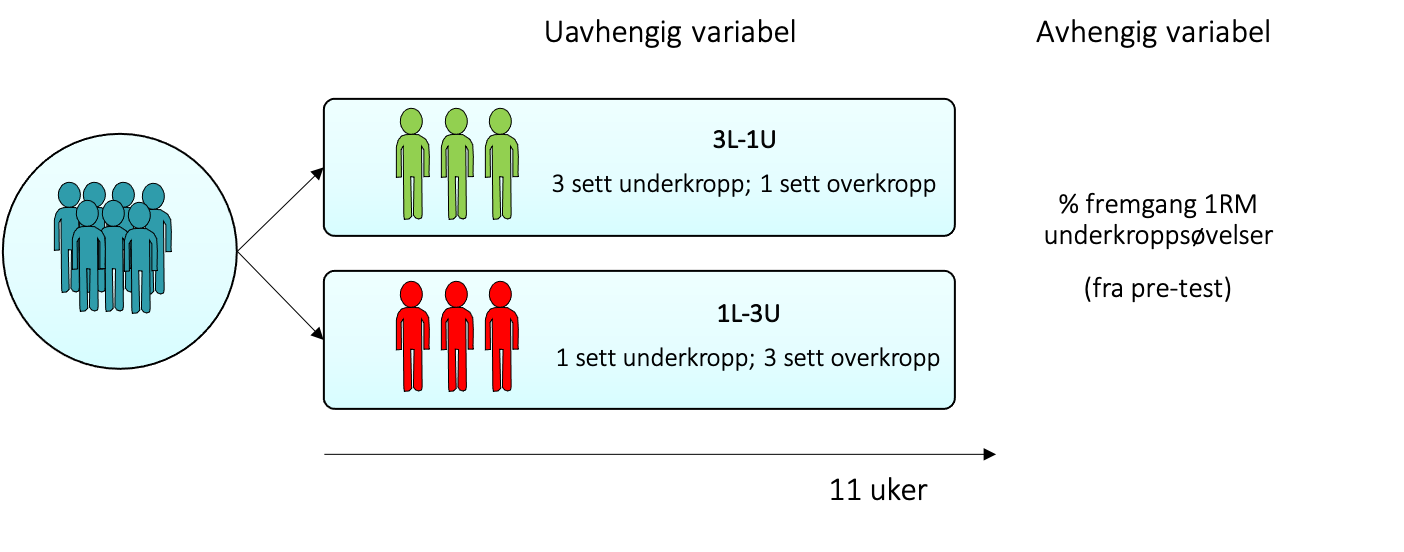
\includegraphics{design.png}
Vi har ikke tilgang til dette datasettet, men jeg har simulert dette datasettet i R basert på verdiene jeg fant i artikkelen. Datasettet blir tilnærmet likt, men siden det er en simulering blir det aldri helt identisk. Datasettet ser du i tabellen under.

\begin{Shaded}
\begin{Highlighting}[]
\NormalTok{knitr}\SpecialCharTok{::}\FunctionTok{kable}\NormalTok{(}
\NormalTok{  dat, }\AttributeTok{booktabs =} \ConstantTok{TRUE}\NormalTok{,}
  \AttributeTok{caption =} \StringTok{\textquotesingle{}Simulert datasett\textquotesingle{}}
\NormalTok{)}
\end{Highlighting}
\end{Shaded}

\begin{table}

\caption{\label{tab:unnamed-chunk-3}Simulert datasett}
\centering
\begin{tabular}[t]{rlr}
\toprule
individ & gruppe & rm\\
\midrule
1 & tre.sett & 40.46704\\
2 & tre.sett & 49.07223\\
3 & tre.sett & 47.94131\\
4 & tre.sett & 44.51389\\
5 & tre.sett & 52.28750\\
\addlinespace
6 & tre.sett & 40.01750\\
7 & tre.sett & 49.48425\\
8 & tre.sett & 29.21048\\
9 & tre.sett & 40.59293\\
10 & tre.sett & 37.58676\\
\addlinespace
11 & tre.sett & 35.42651\\
12 & tre.sett & 42.49354\\
13 & ett.sett & 17.70576\\
14 & ett.sett & 17.07181\\
15 & ett.sett & 18.26811\\
\addlinespace
16 & ett.sett & 25.42594\\
17 & ett.sett & 32.70313\\
18 & ett.sett & 19.10226\\
19 & ett.sett & 22.23827\\
20 & ett.sett & 22.27148\\
\addlinespace
21 & ett.sett & 26.17889\\
22 & ett.sett & 20.34857\\
23 & ett.sett & 23.52773\\
24 & ett.sett & 17.95966\\
\bottomrule
\end{tabular}
\end{table}

Du kan få nøyaktig samme datsett ved å klippe ut og lime inn følgende kode i en skript-fil i R (husk å laste inn tidyverse-pakken, library(tidyverse) ). Du kan også laste ned datasettet som en .csv fil fra canvas.

\begin{Shaded}
\begin{Highlighting}[]
\FunctionTok{set.seed}\NormalTok{(}\DecValTok{2002}\NormalTok{) }\CommentTok{\#viktig å ha med denne for å få nøyaktig samme datasett}
\NormalTok{tre.sett }\OtherTok{\textless{}{-}} \FunctionTok{rnorm}\NormalTok{(}\AttributeTok{n =} \DecValTok{12}\NormalTok{, }\AttributeTok{mean =} \DecValTok{41}\NormalTok{, }\AttributeTok{sd =} \DecValTok{5}\NormalTok{) }\CommentTok{\#12 individer}
\NormalTok{ett.sett }\OtherTok{\textless{}{-}}\FunctionTok{rnorm}\NormalTok{(}\AttributeTok{n =} \DecValTok{12}\NormalTok{, }\AttributeTok{mean =} \DecValTok{21}\NormalTok{, }\AttributeTok{sd =} \DecValTok{5}\NormalTok{) }\CommentTok{\#12 individer}

\CommentTok{\#lager en tibble fra tidyverse{-}pakken. Må ha lastet inn tidyverse library(tidyverse) i scriptfilen}
\NormalTok{dat }\OtherTok{\textless{}{-}} \FunctionTok{tibble}\NormalTok{(}\AttributeTok{individ =} \FunctionTok{seq}\NormalTok{(}\DecValTok{1}\SpecialCharTok{:}\DecValTok{24}\NormalTok{),}
              \AttributeTok{gruppe =} \FunctionTok{rep}\NormalTok{(}\FunctionTok{c}\NormalTok{(}\StringTok{"tre.sett "}\NormalTok{, }\StringTok{"ett.sett"}\NormalTok{), }\FunctionTok{c}\NormalTok{(}\FunctionTok{length}\NormalTok{(tre.sett), }\FunctionTok{length}\NormalTok{(ett.sett))),}
              \AttributeTok{rm =} \FunctionTok{c}\NormalTok{(tre.sett , ett.sett))}
\end{Highlighting}
\end{Shaded}

Før du går videre er det greit at du gjør deg kjent med datasettet som vi har generert. Studer datasettet og svar på følgende spørsmål:

\begin{enumerate}
\def\labelenumi{\arabic{enumi}.}
\tightlist
\item
  Hvor mange kolonner er det i tabellen over?
\item
  Hvor mange deltakere var med i studien?
\item
  Hvilke to verdier kan variabelen gruppe? og
\end{enumerate}

\hypertarget{regne-gjennomsnitt-for-de-to-gruppene}{%
\subsection{Regne gjennomsnitt for de to gruppene}\label{regne-gjennomsnitt-for-de-to-gruppene}}

Bra! Det er alltid viktig å bli kjent med sitt eget datasett, men nå som du har det kan vi gå videre. Vi er interessert i om det er forskjeller mellom de to gruppene (``tre.sett'' vs.~ett.sett) på \% fremgang fra pre- til post-test. Så kanskje vi kan starte med å se om det er forskjeller i gjennomsnitt mellom to gruppene? Dette kan enkelt gjøres i R, Jamovi eller excel. Her er en kode for å gjøre dette i R:

\begin{Shaded}
\begin{Highlighting}[]
\CommentTok{\#jeg lager et oobjekt som heter mean\_rm }
\NormalTok{mean\_rm }\OtherTok{\textless{}{-}}\NormalTok{ dat }\SpecialCharTok{\%\textgreater{}\%}
  \CommentTok{\#Jeg grupperer etter gruppe, slik at jeg får et mean for hver gruppe istf. for å få mean for alle individene}
  \CommentTok{\#group\_by er en funksjon for dette}
  \FunctionTok{group\_by}\NormalTok{(gruppe) }\SpecialCharTok{\%\textgreater{}\%}
  \CommentTok{\#deretter bruker jeg summarise funksjonen for å regne gjennomsnitt}
  \FunctionTok{summarise}\NormalTok{(}\AttributeTok{mean.fremgang.1RM =} \FunctionTok{mean}\NormalTok{(rm))}
\end{Highlighting}
\end{Shaded}

Koden gir oss følgende tabell:
\textbackslash begin\{table\}

\textbackslash caption\{\label{tab:unnamed-chunk-6}Gjennomsnittlige \%-vis fremgang for de to gruppene\}
\centering

\begin{tabular}[t]{lr}
\toprule
gruppe & mean.fremgang.1RM\\
\midrule
ett.sett & 21.90013\\
tre.sett & 42.42450\\
\bottomrule
\end{tabular}

\textbackslash end\{table\}

Hvilken gruppe hadde mest fremgang?
mcq(c(``ett.sett'', answer = ``tre.sett''))

\hypertarget{figur-av-datasettet}{%
\subsection{Figur av datasettet}\label{figur-av-datasettet}}

Vi kan også presentere dataen i en figur. En vanlig måte å gjøre dette på er å bruke et stolpediagram.

\begin{figure}

{\centering 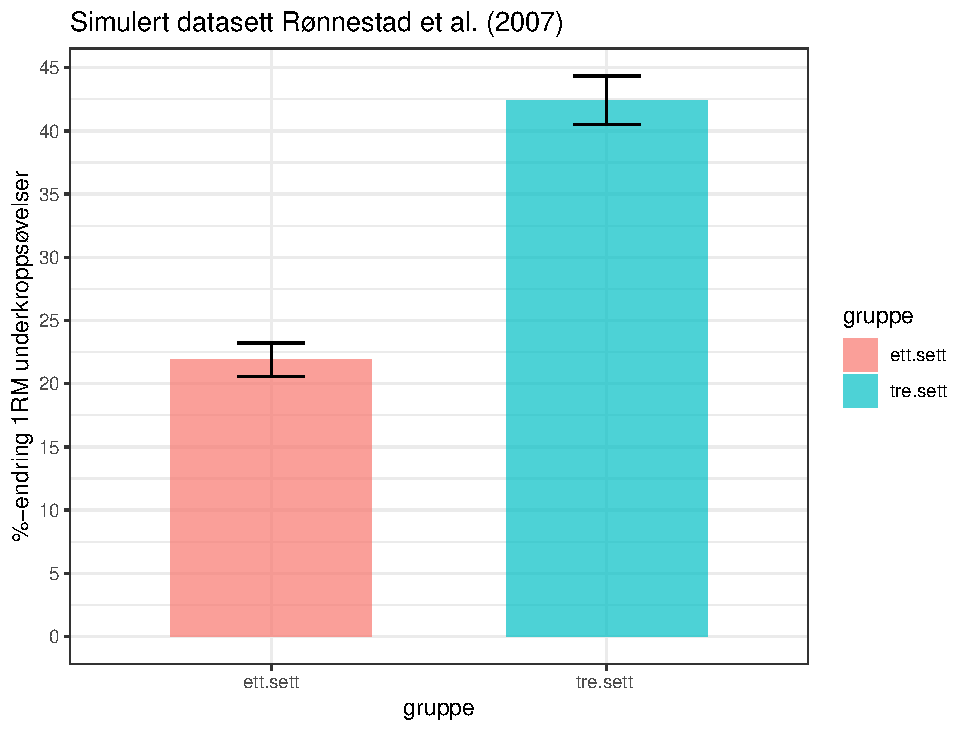
\includegraphics[width=0.8\linewidth]{bok_files/figure-latex/nice-fig-1} 

}

\caption{Here is a nice figure!}\label{fig:nice-fig}
\end{figure}

Et stolpediagram er pent å se på, men er egentlig designet for kategorisk data. For eksempel er det fint å bruke dette når vi skal presentere frekvensen antall som har kjørt bil til skolen og antall personer som har gått. Les \href{https://journals.plos.org/plosbiology/article?id=10.1371/journal.pbio.1002128}{Beyond Bar and Line Graphs: Time for a New Data Presentation Paradigm}, og svar på følgende spørsmål:

\begin{Shaded}
\begin{Highlighting}[]
\NormalTok{knitr}\SpecialCharTok{::}\FunctionTok{include\_app}\NormalTok{(}\StringTok{"https://cmagelssen.shinyapps.io/test/"}\NormalTok{, }
  \AttributeTok{height =} \StringTok{"600px"}\NormalTok{)}
\end{Highlighting}
\end{Shaded}

\begin{verbatim}
## PhantomJS not found. You can install it with webshot::install_phantomjs(). If it is installed, please make sure the phantomjs executable can be found via the PATH variable.
\end{verbatim}

\hypertarget{hvilken-modell-skal-vi-velge}{%
\chapter{Hvilken modell skal vi velge?}\label{hvilken-modell-skal-vi-velge}}

Her tenker jeg å si litt om at vi har ulike muligheter.

\hypertarget{h0-null-hypotese}{%
\chapter{H0: Null-hypotese}\label{h0-null-hypotese}}

Her tenker jeg å si at Null-hypotesen er at det ingen forskjeller mellom gruppene. Og at alt vi trenger er å predikere et individs skår med gjennomsnittet for alle individene i hele datasettet.

Deretter regner jeg ut error for alle gruppene.

\hypertarget{h1-alternativ-hypotese}{%
\chapter{H1: Alternativ hypotese}\label{h1-alternativ-hypotese}}

We have finished a nice book.

\hypertarget{f-ratio-og-signifikanstesting}{%
\chapter{f-ratio og signifikanstesting}\label{f-ratio-og-signifikanstesting}}

We have finished a nice book.

\hypertarget{f-tester-i-jamovi}{%
\chapter{F-tester i Jamovi}\label{f-tester-i-jamovi}}

We have finished a nice book.

  \bibliography{book.bib,packages.bib}

\end{document}
